% Open Source Gonioreflectometer -- manuscript for HardwareX (Elsevier). Build: `make paper` (repo root) -> paper/build/opengonio.pdf
% Structure: HardwareX hardware-article template. Citations: APA 7 (biblatex-apa); keys = IDs in REFERENCES.md.
% Tables in generated/ and figures in figures/ come from the repo (tools/paper_assets.py): do not edit them by hand.
% SPDX-License-Identifier: CC-BY-SA-4.0
\documentclass[preprint,12pt,nonatbib]{elsarticle}
\usepackage[T1]{fontenc}
\usepackage[utf8]{inputenc}
\usepackage[american]{babel}
\usepackage{csquotes}
\makeatletter\let\c@author\relax\makeatother   % elsarticle and biblatex both define the author counter
\usepackage[style=apa,backend=biber]{biblatex}
\addbibresource{references.bib}
\usepackage{amsmath,amssymb,graphicx,tabularx,longtable,booktabs,xcolor,siunitx}
\usepackage[hidelinks]{hyperref}
\hypersetup{pdftitle={Open Source Gonioreflectometer: a four-axis BRDF instrument and 3D scanner built from printed parts without soldering},
  pdfauthor={Aleksander Norman}, pdfsubject={Open-source scientific hardware},
  pdfkeywords={BRDF, gonioreflectometer, material appearance, open hardware, 3D printing}, pdflang={en-US}}
\usepackage{url}
\graphicspath{{figures/}}
% generated by tools/paper_assets.py
\newcommand{\costparts}{US\$495.19}
\newcommand{\costtools}{US\$469.76}
\newcommand{\nprinted}{56}
\newcommand{\nbought}{48}
\newcommand{\abs}{2664}

\newcommand{\tbd}[1]{\textcolor{red}{\textbf{[TBD: #1]}}}   % placeholder until measured data exists

\ifdefined\pdftrailerid\pdftrailerid{opengonio}\fi   % same source -> same PDF bytes (no noise in git)
\journal{HardwareX}

\begin{document}
\begin{frontmatter}
\title{Open Source Gonioreflectometer: a four-axis BRDF instrument and 3D scanner built from printed parts without soldering}

\author[csudh]{Aleksander Norman\corref{cor}}
\cortext[cor]{Corresponding author: \tbd{email}}
\affiliation[csudh]{organization={California State University, Dominguez Hills},
  city={Carson}, state={CA}, country={USA}}

\begin{abstract}
The Open Source Gonioreflectometer measures the bidirectional reflectance distribution function (BRDF) of flat samples and scans objects in 3D.
A light arm on a \SI{305}{mm} ring and three sample axes (yaw, tilt, spin) set every illumination and viewing direction
relative to a fixed camera, following \textcite{R1}. All \nprinted{} structural parts are 3D printed in ABS; the
\nbought{} bought parts cost \costparts{} from three distributors. No soldering, drilling, sawing or crimping is needed.
Calibration uses a mirror for angles, an exposure series for camera response and a pressed-PTFE tile for absolute
reflectance. Fitted Lambert + GGX parameters export to game engines. \tbd{repeatability, accuracy vs. reference data}.
\end{abstract}

\begin{keyword}
BRDF \sep gonioreflectometer \sep material appearance \sep open hardware \sep 3D printing \sep photometric calibration
\end{keyword}
\end{frontmatter}

\section*{Specifications table}
% generated by tools/paper_assets.py
\begin{tabularx}{\linewidth}{|l|X|}\hline
Hardware name & Open Source Gonioreflectometer \\ \hline
Subject area & Engineering and materials science; computer graphics (material appearance) \\ \hline
Hardware type & Measuring physical properties and in-lab sensors; imaging tools \\ \hline
Closest commercial analog & Laboratory gonioreflectometers and goniospectrophotometers \\ \hline
Open source license & Hardware CERN-OHL-S-2.0; software GPL-3.0-or-later; documentation CC BY-SA 4.0 \\ \hline
Cost of hardware & US\$569.10 in parts (cap US\$630); tools US\$469.76 \\ \hline
Source file repository & \url{https://github.com/Normansrule/Gonioreflectometer-Open-Source} (DOI at release) \\ \hline
\end{tabularx}


\section{Hardware in context}
Gonioreflectometers measure how a surface reflects light as a function of incident and reflected direction
\parencite{G1}. Laboratory instruments reach high accuracy at high cost \parencite{G25,G27,G31}; image-based
\parencite{G12,G15} and robot-arm \parencite{G39} setups lower the cost but still need machining or industrial arms.
Consumer-hardware capture \parencite{G38} trades angular coverage for speed. \textcite{R1} describe a multispectral
goniometric device with a light arm and a three-axis sample stage. The Open Source Gonioreflectometer reproduces that geometry with printed parts,
stepper motors and a USB camera, for builders without a workshop, consistent with open-hardware practice
\parencite{H28,H34}.

\section{Hardware description}
\begin{figure}[h]\centering
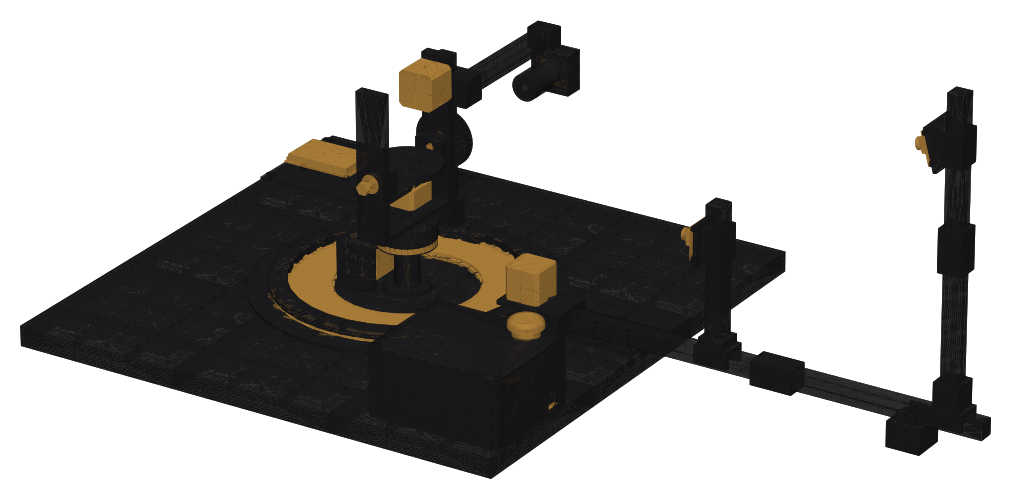
\includegraphics[width=0.85\linewidth]{assembly.png}
\caption{Whole-machine assembly from the repository CAD (\texttt{cad/assembly}). Sample axes at centre, light arm on the
ring, measuring camera on the right.}\label{fig:assembly}
\end{figure}

\begin{figure}[h]\centering
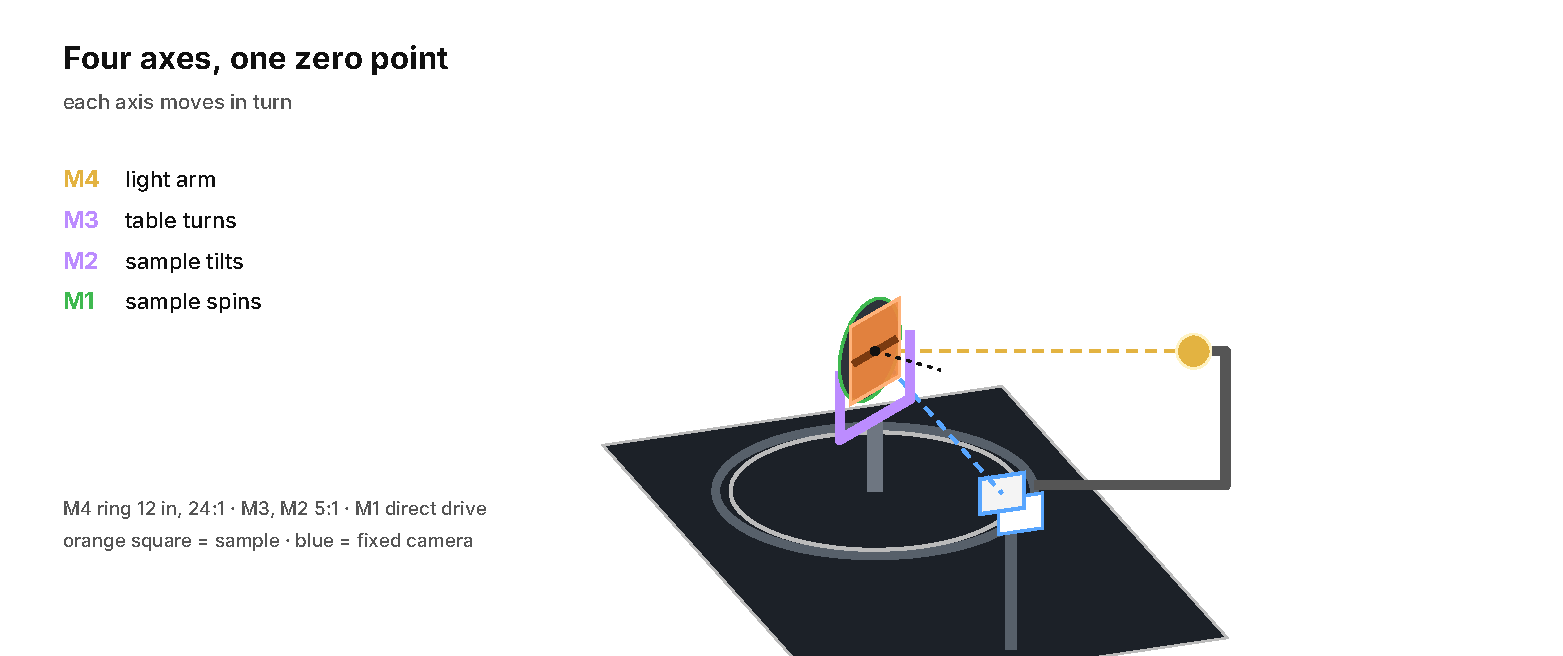
\includegraphics[width=\linewidth]{axes.pdf}
\caption{Four axes, one zero point. M4: light arm; M3: table yaw; M2: tilt; M1: spin.}\label{fig:axes}
\end{figure}

\begin{itemize}
\item \textbf{Geometry.} M4 (light arm, 20--324\textdegree, 24:1 belt on the ring), M3 (yaw, $\pm$180\textdegree, 5:1),
  M2 (tilt, $\pm$90\textdegree, 5:1), M1 (spin, direct drive). Camera fixed at \SI{350}{mm}; light at \SI{300}{mm}
  (Fig.~\ref{fig:axes}). Anisotropic materials need M1 \parencite{G9}.
\item \textbf{Light.} Chip-on-board LED, colour rendering index 97, \SI{350}{mA} constant current, collimating printed
  tube with a \SI{10}{mm} aperture; solderless holder clamped by the lamp body.
\item \textbf{Camera.} 12 MP IMX477 USB module, \SI{16}{mm} lens, printed f/8 stop; exposure, gain and white balance locked.
\item \textbf{Control.} grblHAL on an RP2040 board (BTT SKR Pico, USB-C) drives four steppers; a microcontroller reads keypads and sensors;
  optical homing on every axis; over-travel switches in the emergency-stop loop.
\item \textbf{One screw size.} Every printed join and module mount is an M2 screw self-tapping into a printed pilot;
  M3 only into the motors, M8 bolts as axles. The base is a printed deck of nine tiles with a pilot at every mount point.
\item \textbf{No-tool joins.} Lever connectors, screw terminals and modules (optocoupler, LED driver) instead of loose chips.
\end{itemize}

\section{Design files summary}
% generated by tools/paper_assets.py
{\small\begin{longtable}{|p{0.34\linewidth}|l|l|l|}\caption{Design files summary. Printed parts: \texttt{phases/<stage>/3d/}, STEP and STL.}\label{tab:design}\\\hline
\textbf{Design file} & \textbf{Type} & \textbf{License} & \textbf{Location} \\ \hline\endfirsthead
\hline\textbf{Design file} & \textbf{Type} & \textbf{License} & \textbf{Location} \\ \hline\endhead
PLAN-01 tolerance coupon & STEP, STL & CERN-OHL-S-2.0 & \path{00-plan} \\
PWR-18 power plate & STEP, STL & CERN-OHL-S-2.0 & \path{01-power} \\
CTL-10a button panel & STEP, STL & CERN-OHL-S-2.0 & \path{02-controller} \\
CTL-10b controller tray & STEP, STL & CERN-OHL-S-2.0 & \path{02-controller} \\
FRM-01a deck tile SW & STEP, STL & CERN-OHL-S-2.0 & \path{03-frame} \\
FRM-01b deck tile S & STEP, STL & CERN-OHL-S-2.0 & \path{03-frame} \\
FRM-01c deck tile SE & STEP, STL & CERN-OHL-S-2.0 & \path{03-frame} \\
FRM-01d deck tile W & STEP, STL & CERN-OHL-S-2.0 & \path{03-frame} \\
FRM-01e deck tile C & STEP, STL & CERN-OHL-S-2.0 & \path{03-frame} \\
FRM-01f deck tile E & STEP, STL & CERN-OHL-S-2.0 & \path{03-frame} \\
FRM-01g deck tile NW & STEP, STL & CERN-OHL-S-2.0 & \path{03-frame} \\
FRM-01h deck tile N & STEP, STL & CERN-OHL-S-2.0 & \path{03-frame} \\
FRM-01i deck tile NE & STEP, STL & CERN-OHL-S-2.0 & \path{03-frame} \\
FRM-02a outrigger bar 1 & STEP, STL & CERN-OHL-S-2.0 & \path{03-frame} \\
FRM-02b outrigger bar 2 & STEP, STL & CERN-OHL-S-2.0 & \path{03-frame} \\
FRM-02c scan post bar 1 & STEP, STL & CERN-OHL-S-2.0 & \path{03-frame} \\
FRM-02d scan post bar 2 & STEP, STL & CERN-OHL-S-2.0 & \path{03-frame} \\
FRM-09c protractor segment & STEP, STL & CERN-OHL-S-2.0 & \path{03-frame} \\
FRM-09d bar saddle & STEP, STL & CERN-OHL-S-2.0 & \path{03-frame} \\
FRM-09e post socket & STEP, STL & CERN-OHL-S-2.0 & \path{03-frame} \\
FRM-09f end foot & STEP, STL & CERN-OHL-S-2.0 & \path{03-frame} \\
FRM-09h camera pillar & STEP, STL & CERN-OHL-S-2.0 & \path{03-frame} \\
FRM-09i bar coupler & STEP, STL & CERN-OHL-S-2.0 & \path{03-frame} \\
LAR-08a rim segment & STEP, STL & CERN-OHL-S-2.0 & \path{04-light-arm} \\
LAR-08b ring motor mount & STEP, STL & CERN-OHL-S-2.0 & \path{04-light-arm} \\
LAR-08c arm segment & STEP, STL & CERN-OHL-S-2.0 & \path{04-light-arm} \\
LAR-08e cross clamp & STEP, STL & CERN-OHL-S-2.0 & \path{04-light-arm} \\
LAR-08f upright bar & STEP, STL & CERN-OHL-S-2.0 & \path{04-light-arm} \\
LAR-08g arm bar & STEP, STL & CERN-OHL-S-2.0 & \path{04-light-arm} \\
TBL-07a table drum & STEP, STL & CERN-OHL-S-2.0 & \path{05-table} \\
TBL-07b home flag & STEP, STL & CERN-OHL-S-2.0 & \path{05-table} \\
TBL-07c table motor bracket & STEP, STL & CERN-OHL-S-2.0 & \path{05-table} \\
TBL-07d table post & STEP, STL & CERN-OHL-S-2.0 & \path{05-table} \\
TBL-07f spacers & STEP, STL & CERN-OHL-S-2.0 & \path{05-table} \\
TBL-07g endstop riser & STEP, STL & CERN-OHL-S-2.0 & \path{05-table} \\
TBL-07h table flag & STEP, STL & CERN-OHL-S-2.0 & \path{05-table} \\
CAM-03a aperture stop f8 & STEP, STL & CERN-OHL-S-2.0 & \path{06-camera-light} \\
CAM-03b camera plate & STEP, STL & CERN-OHL-S-2.0 & \path{06-camera-light} \\
LSR-05a lamp tube & STEP, STL & CERN-OHL-S-2.0 & \path{06-camera-light} \\
LSR-05b lamp cap & STEP, STL & CERN-OHL-S-2.0 & \path{06-camera-light} \\
CAL-06a ptfe holder & STEP, STL & CERN-OHL-S-2.0 & \path{07-calibrate} \\
CAL-06b mirror holder & STEP, STL & CERN-OHL-S-2.0 & \path{07-calibrate} \\
CAL-06c ball holder & STEP, STL & CERN-OHL-S-2.0 & \path{07-calibrate} \\
ENC-04a dowel socket & STEP, STL & CERN-OHL-S-2.0 & \path{07-calibrate} \\
TLT-07a tilt yoke & STEP, STL & CERN-OHL-S-2.0 & \path{08-tilt} \\
TLT-07b pulley 100T & STEP, STL & CERN-OHL-S-2.0 & \path{08-tilt} \\
TLT-07c tilt cradle & STEP, STL & CERN-OHL-S-2.0 & \path{08-tilt} \\
SPN-07a spin platter & STEP, STL & CERN-OHL-S-2.0 & \path{09-spin} \\
MSK-06a led ring & STEP, STL & CERN-OHL-S-2.0 & \path{10-color} \\
MSK-06b led mast & STEP, STL & CERN-OHL-S-2.0 & \path{10-color} \\
SPC-03a spectral tube & STEP, STL & CERN-OHL-S-2.0 & \path{10-color} \\
SCN-03a riser 20 & STEP, STL & CERN-OHL-S-2.0 & \path{11-scan-capture} \\
SCN-03b riser 40 & STEP, STL & CERN-OHL-S-2.0 & \path{11-scan-capture} \\
SCN-03c riser 60 & STEP, STL & CERN-OHL-S-2.0 & \path{11-scan-capture} \\
SCN-03d scan camera plate 15 & STEP, STL & CERN-OHL-S-2.0 & \path{11-scan-capture} \\
STA-07a pi zero mount & STEP, STL & CERN-OHL-S-2.0 & \path{15-standalone} \\
Bought-part stand-ins & STEP, STL & CERN-OHL-S-2.0 & \path{cad/bought} \\
Whole-machine assembly & STEP & CERN-OHL-S-2.0 & \path{cad/assembly} \\
CAD source (CadQuery) & Python & GPL-3.0-or-later & \path{tools/cad} \\
\hline\end{longtable}}


\section{Bill of materials summary}
Parts from Digi-Key, Amazon and Adafruit. Tools (\costtools{}, including the printer) are listed separately in the
repository. Printed parts: $\approx$\SI{\abs}{g} ABS.
% generated by tools/paper_assets.py
{\small\begin{longtable}{|l|p{0.43\linewidth}|r|r|r|l|}\caption{Bill of materials summary (core machine; shared packs counted once; prices in USD, checked on the store pages).}\label{tab:bom}\\\hline
\textbf{Designator} & \textbf{Component} & \textbf{No.} & \textbf{Unit} & \textbf{Total} & \textbf{Source} \\ \hline\endfirsthead
\hline\textbf{Designator} & \textbf{Component} & \textbf{No.} & \textbf{Unit} & \textbf{Total} & \textbf{Source} \\ \hline\endhead
FIL-01 & ABS filament 1.75 mm, black, 1 kg (2 spools) & 2 & 15.99 & 31.98 & Amazon \\
PWR-01 & AC adapter 24 V 2.5 A 60 W & 1 & 35.26 & 35.26 & Digi-Key \\
PWR-02 & IEC C13 mains cord & 1 & 3.14 & 3.14 & Amazon \\
PWR-03 & DC jack to screw-terminal adapter 2.1 mm & 1 & 2.00 & 2.00 & Adafruit \\
PWR-04 & Inline 5 x 20 mm fuse holder & 1 & 4.00 & 4.00 & Digi-Key \\
PWR-05 & Fuse 3.15 A time-lag 5 x 20 mm & 2 & 1.56 & 3.12 & Digi-Key \\
PWR-10 & Optocoupler LTV-817 / PC817 (DIP-4) & 1 & 0.39 & 0.39 & Digi-Key \\
PWR-11 & Resistors 10k (2) & 2 & 0.10 & 0.20 & Digi-Key \\
PWR-13 & Emergency stop 22 mm latching, 1 NC & 1 & 30.87 & 30.87 & Digi-Key \\
PWR-15 & 18 AWG silicone wire red/black, 1 m pair & 1 & 7.98 & 7.98 & Amazon \\
PWR-19 & Half-size breadboard (400 points) & 1 & 4.95 & 4.95 & Adafruit \\
PWR-20 & Lever wire connectors, WAGO 221 assortment (12) & 1 & 12.45 & 12.45 & Amazon \\
CTL-01 & FYSETC E4 (ESP32, 4x TMC2209, WiFi + Bluetooth) & 1 & 40.99 & 40.99 & Amazon \\
CTL-02 & Raspberry Pi Pico H (headers soldered) & 1 & 5.00 & 5.00 & Digi-Key \\
CTL-03 & USB A-to-B cable for the E4 & 1 & 3.95 & 3.95 & Adafruit \\
CTL-04 & USB-A to micro-B data cable 1 m & 1 & 2.95 & 2.95 & Adafruit \\
CTL-05 & Membrane keypad 1 x 4 & 2 & 2.95 & 5.90 & Adafruit \\
CTL-06 & JST-XH pre-crimped lead kit & 1 & 10.99 & 10.99 & Amazon \\
CTL-07 & Jumper wires male-female 150 mm (20) & 2 & 1.95 & 3.90 & Adafruit \\
CTL-11 & Stepper cables 1 m, PH2.0 6-pin to XH2.54 4-pin (4-pack) & 1 & 6.00 & 6.00 & Amazon \\
FRM-01 & Baltic birch plywood 1/2 in, 24 x 24 in & 1 & 20.00 & 20.00 & Amazon \\
FRM-02 & 2020 V-slot 500 mm (4-pack) & 1 & 22.39 & 22.39 & Amazon \\
FRM-03 & M5 T-nuts for 2020, 50 drop-in + 50 sliding & 1 & 5.99 & 5.99 & Amazon \\
FRM-06 & Socket screw kit M2–M5, 8/10/16/20 mm, with nuts & 1 & 9.99 & 9.99 & Amazon \\
FRM-08 & 608-2RS bearings (10) & 1 & 4.99 & 4.99 & Amazon \\
FRM-12 & Wood screws \#8 x 5/8 in, Type 17 point (100) & 1 & 8.60 & 8.60 & Amazon \\
LAR-01 & 12 in lazy Susan bearing & 1 & 13.99 & 13.99 & Amazon \\
LAR-02 & NEMA 17 stepper 59 Ncm 2 A (3-pack: M4, M3, M2) & 1 & 32.99 & 32.99 & Amazon \\
LAR-03 & GT2 6 mm open belt (5 m) & 1 & 7.59 & 7.59 & Amazon \\
LAR-04 & GT2 20T pulley 5 mm bore (5-pack) & 1 & 3.99 & 3.99 & Amazon \\
LAR-05 & Optical endstop module, slot type (6-pack) & 1 & 8.99 & 8.99 & Amazon \\
LAR-06 & Roller-lever limit switch, screw terminals (2) & 1 & 6.99 & 6.99 & Amazon \\
TBL-02 & GT2 6 mm closed belt 232 mm & 1 & 8.19 & 8.19 & Amazon \\
TBL-05 & M8 x 75 hex bolt, partial thread + M8 nut (fixed table axle) & 1 & 15.37 & 15.37 & Amazon \\
CAM-01 & USB camera 12 MP IMX477, M12 mount (UVC) & 1 & 59.99 & 59.99 & Amazon \\
CAM-02 & M12 lens 16 mm, $\geq$ 1/2 in format, low distortion & 1 & 30.11 & 30.11 & Amazon \\
LSR-06 & Solderless COB holder 13.5 mm (TE LUMAWISE Z35) & 1 & 3.50 & 3.50 & Digi-Key \\
CAM-07 & M2.5 x 8 mm screws (100-pack) & 1 & 6.29 & 6.29 & Amazon \\
LSR-01 & COB LED CRI 97, 12 V, 13.5 mm (Citizen CLU7A3) & 1 & 5.91 & 5.91 & Digi-Key \\
LSR-02 & Constant-current driver 350 mA & 1 & 5.41 & 5.41 & Digi-Key \\
LSR-03 & Heatsink 40 x 40 mm (from a pack) & 1 & 6.99 & 6.99 & Amazon \\
ENC-02 & Black felt sheet & 1 & 6.99 & 6.99 & Amazon \\
CAL-01 & PTFE sheets 100 x 100 x 3 mm (2): white tile = 3 stacked 50 mm squares & 1 & 16.99 & 16.99 & Amazon \\
CAL-02 & Glass mirror tile \textasciitilde{}50 mm & 1 & 11.49 & 11.49 & Amazon \\
CAL-04 & ChArUco print + picture-frame glass & 1 & 4.31 & 4.31 & Amazon \\
TLT-02 & GT2 6 mm closed belt 280 mm & 1 & 7.49 & 7.49 & Amazon \\
TLT-05 & M8 x 35 hex bolts, half thread (10-pack; 2 used) & 1 & 9.19 & 9.19 & Amazon \\
SPN-01 & NEMA 17 pancake stepper 16 Ncm 1 A (direct drive) & 1 & 11.99 & 11.99 & Amazon \\
SCN-01 & Mounting putty 2 oz & 1 & 2.33 & 2.33 & Amazon \\
SCN-02 & ChArUco scanning mat print & 1 & 1.00 & 1.00 & print shop / library (service) \\
\hline\multicolumn{4}{|r|}{\textbf{Total}} & \textbf{576.06} & \multicolumn{1}{l|}{} \\ \hline
\end{longtable}}


\section{Build instructions}
The repository splits the build into stages (power, controller, frame, each axis, camera and light, calibration).
Each step lists time, parts, actions, a measured pass criterion and what to check on failure (\path{phases/*/README.md}).
\begin{enumerate}
\item Print the tolerance coupon; set clearance and self-tap hole size.
\item Wire the power box; check polarity and fuse before the first power-on.
\item Mount the controller; move one motor from the laptop.
\item Print and bolt the deck; screw every mount into its pilot; assemble the axes; home each axis.
\item Mount camera and lamp; run the mirror test; calibrate (Section~\ref{sec:validation}).
\end{enumerate}

\section{Operation instructions}
\begin{enumerate}
\item \texttt{opengonio check-pose M4=60 M3=30}: angle and collision check.
\item \texttt{opengonio capture inplane --step 10 --out data/s}: in-plane sweep.
\item \texttt{opengonio curve data/s}: calibrated BRDF curve and Lambert + GGX fit \parencite{R6,T11}.
\end{enumerate}
Safety: the lamp is viewed only through the sample; the emergency stop cuts motor power.

\section{Validation and characterization}\label{sec:validation}
\paragraph{Calibration.} Angle offset from the mirror peak ($M_3 = M_4/2$ in-plane); dark level from a lamp-off frame;
camera response from an exposure series \parencite{R5}; absolute scale from pressed PTFE \parencite{N30}:
\begin{equation}
f_r=\frac{C_{\mathrm{lin}}}{C_{w,\mathrm{lin}}}\,\frac{\rho_w}{\pi}\,\frac{\cos 45^\circ}{\cos\theta_i},\qquad
C_{\mathrm{lin}}=(C-C_d)^{\gamma}.
\end{equation}
\paragraph{Results.} \tbd{angular repeatability per axis (mirror, 10 repeats); lamp drift over a run; PTFE reflectance
vs. reference; matte and glossy samples vs. MERL \parencite{G15} or RGL \parencite{R16} data; scan accuracy}.

\section*{Ethics statements}
No human or animal subjects.

\section*{CRediT author statement}
\textbf{Aleksander Norman:} Conceptualization, Methodology, Software, Hardware, Writing -- original draft.

\section*{Declaration of competing interest}
None.

\section*{Acknowledgements}
\tbd{acknowledgements}

\printbibliography
\end{document}
